\documentclass{article}
\newcommand{\exptitle}{Flammersfield Oscillator}
\newcommand{\course}{PHYS3113 - Thermodynamics and Statistical Mechanics}

\usepackage{graphicx}
\usepackage{pgf}
\usepackage{lmodern}
\usepackage{import}
\usepackage{booktabs}
\usepackage{tabu}
\usepackage{float}
\usepackage[hidelinks]{hyperref}
\usepackage{amsmath}
\usepackage{amsfonts}
\usepackage[margin=1in]{geometry}
\usepackage{pythonhighlight}
\usepackage[toc]{appendix}
\usepackage{float}
\usepackage{placeins}
\usepackage{natbib}
\usepackage{lmodern}
\usepackage{subfig}
\usepackage[utf8]{inputenc}
\usepackage[T1]{fontenc}
\usepackage{upgreek}
\usepackage{chemmacros}
\usepackage{braket}
\usepackage{newpxtext,newpxmath}
\usepackage{tikz}

\DeclareMathOperator{\sech}{sech}
\DeclareMathOperator{\cosech}{cosech}

\setlength{\parskip}{1em}
\setlength{\parindent}{0em}

\begin{document}

\begin{titlepage}
    \begin{center}
        \vspace*{7cm}

        \Huge
        \textbf{\exptitle}

        \vspace{0.5cm}
        \LARGE
        \course

        \vspace{1.5cm}

        \textbf{Toby Nguyen - z5416116}
    \end{center}
\end{titlepage}

\tableofcontents


\section{Introduction}
The Flammersfeld oscillator is an improvement upon the Ruchardt Experiment. The 
prior set out to find the molar heat capacities of gas and consequently was able 
to yield also the adiabatic index of gas. Flammersfeld improved upon the established 
experiment by fixing its friction and gas leaks issues. The main idea of the set up is 
that the gas is compressed adiabatically, increasing the temperature of the gas inside
and so the expansion of the gas allows for the calculation of the adiabatic constant.

\section{Method}

\subsection{Experimental Setup}

\begin{figure} [H]
    \centering
    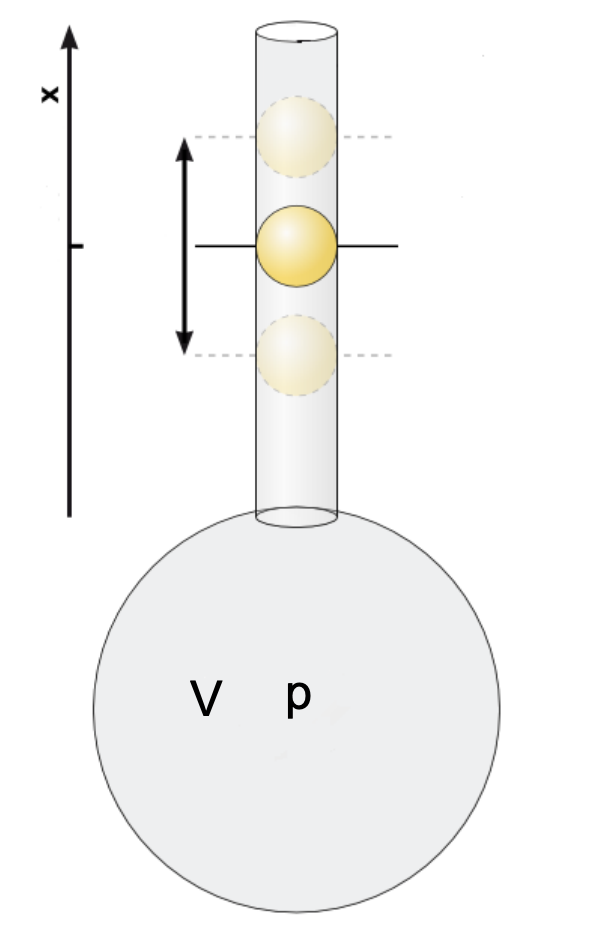
\includegraphics[width = 0.4\textwidth]{../Figures/simplediagram.png}
    \caption{Simple diagram of the experimental setup. The narrow neck bottle is filled with gas. The cylinder 
    of mass $m$ corks the bottle. The volume of the reservoir when the cork is not moving i.e equilibrium is $V$.}
    \label{fig:simplediagram}
\end{figure}

The volume of the flask is $V=1.155$ L and the oscillator radius is $5.95\times10^{-3}$ m. The activation energy 
of bending vibrations $\hbar \omega = 960K$

For all three experiments, gas was pumped into the bottle until there was enough pressure to raise the cork into 
the position found in Figure \ref{fig:simplediagram}. The pressure was slightly changed to induce a disturbance to 
cause the cork to start bobbing up and down. The counting of oscillation was done by a fork light barrier.

\subsection{Theory}
From Figure \ref{fig:simplediagram}, the equilibrium pressure will be 

\begin{equation}
    P = P_0 + \frac{mg}{\pi r^2}
\end{equation}

where $P_0$ is the atmospheric pressure, $r$ is the radius of the bottle neck and $g$ is the acceleration due to 
gravity in free fall. If we let $x(t)$ be a small displacement of the cork from its equilibrium position, then the 
equation of frictionless motion is 

\begin{equation}
    m\frac{d^2x}{dt^2} = \pi r^2 \delta P(x)
\end{equation}

where $\delta P(x)$ is the difference of internal gas pressure form the equilibrium value $P$ when the cylinder's 
displacement is $x$. Consider small oscillations when $\delta P \ll P$, to find $\delta P(x)$, we will differentiate 
the adiabatic equation,

\begin{equation}
    PV^{\chi} = const
\end{equation}

where $\chi$ is the adiabatic coefficient. Hence,

\begin{equation}
    \delta P(x) = - \chi P \frac{\delta V(x)}{V}
\end{equation}

where $\delta V(x)=\pi r^2 x$ is the change of volume after the cork's displacement. Defining frequency, $\Omega$,

\begin{equation}
    \Omega \equiv \pi r^2 \sqrt{\frac{\chi P}{m V}}.
\end{equation}

We can then rewrite the equation of motion to be 

\begin{align}
    m\frac{d^2x}{dt^2} &= \pi r^2 \delta P(x) \\
    \frac{d^2x}{dt^2} &= \frac{\pi r^2}{m} (-\chi P\frac{\delta V(x)}{V}) \\
    &= \frac{\pi r^2}{m} (-\chi P\frac{\pi r^2 x}{V}).
\end{align}

We eventually obtain

\begin{equation}
    \frac{d^2x}{dt^2} + \Omega^2 x(t) = 0.
\end{equation}

If we define a period of motion, $\tau$,

\begin{equation}
    \tau \equiv \frac{2\pi}{\Omega}.
\end{equation}

We will obtain another formula for the adiabatic coefficient,

\begin{equation} \label{eqn: main}
    \chi = \frac{4mV}{P r^4 \tau^2}.
\end{equation}

For one vibrational mode with excitation frequency $\omega$, any integer number of quanta of this 
vibration can be created. However to thermally excite these quanta, there more quanta created, the 
more energy is required and these high energy excitations are suppressed by a Boltzmann factor 
$e^{\frac{E_n}{T}}$ where $E_n = n\omega$ is the energy of $n$ quanta and $T$ is the temperature.

The average vibrational energy is 

\begin{equation}
    E_v(\omega,T) = -\frac{\partial \ln(Z)}{\partial \beta} = \frac{\omega}{e^{\frac{\omega}{T}}-1}
\end{equation}

where $\beta = \frac{1}{T}$. The vibrational contribution to heat capacity is then 

\begin{equation} \label{eqn:1}
    \delta C_V = \frac{\partial E_v(\omega, T)}{\partial T} = \frac{\omega^2}{T^2}\frac{e^{\frac{\omega}{T}}}{(e^{\frac{\omega}{T}}-1)^2}.
\end{equation}

At small temperatures $T \ll \omega$, the vibrational contribution vanishes exponentially, $\delta C_V \approx \frac{\omega^2}{T^2}e^{\frac{-\omega}{T}}$.
At big temperatures $T \gg \omega$, $\delta C_V \approx 1$. Comparing it to $C_V = \frac{f}{2}$, we find that each unfrozen vibrational mode yields 
2 degrees of freedom.

To extract an experimental value of $\delta C_V$, we will consider 

\begin{equation}
    C_V = C_V^{(0)} + \delta C_V 
\end{equation}

where $C_V^{(0)} = \frac{5}{2}$ is the heat capacity without any vibrational contribution, so

\begin{equation} \label{eqn:2}
    \delta C_V = \frac{1}{\chi - 1} - \frac{5}{2}.
\end{equation}

\begin{figure} [H]
    \centering
    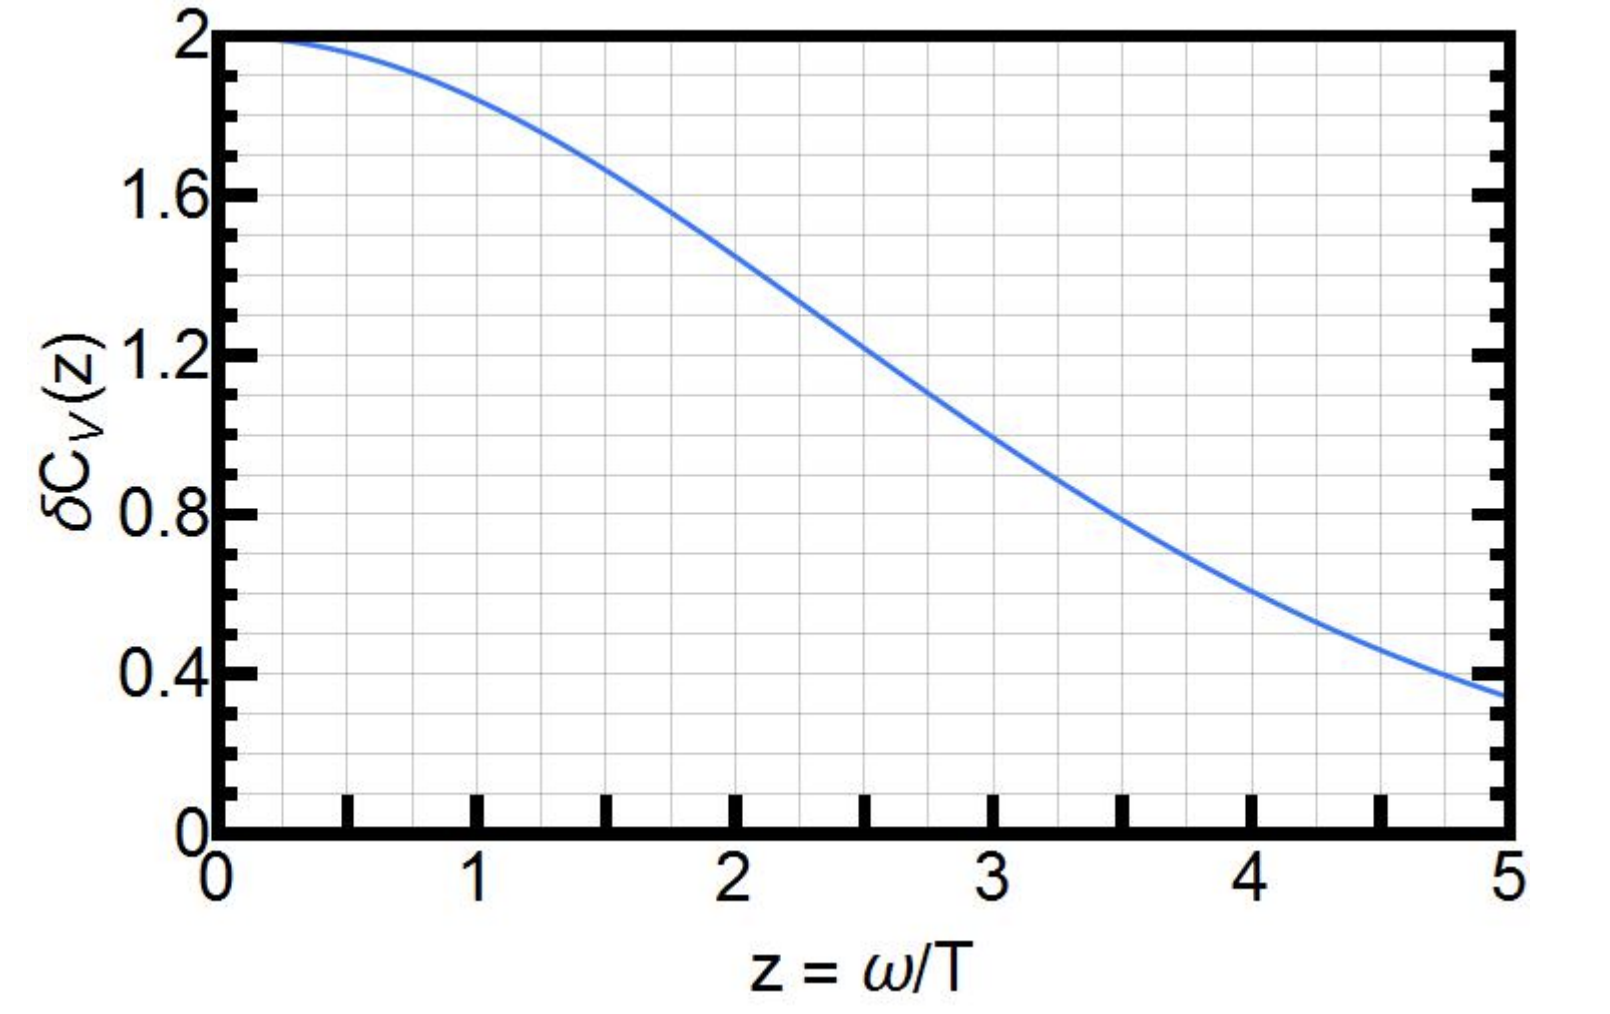
\includegraphics[width=0.8\textwidth]{../Figures/convert.png}
    \caption{Graph of $\delta C_V$ as a function of $\frac{\omega}{T}$ as found in Equation \ref{eqn:1}}
    \label{fig:graph}
\end{figure}

We can then use Figure \ref{fig:graph} to convert our experimental $\delta C_V$ value into an excitation energy, 
$\frac{\omega}{T}$.

\subsection{Erlang distribution}
Since we are measuring the time it takes for number of oscillations, $k$, which is inherently a Poisson process, 
we can model the distribution of different trials as an Erlang distribution. An Erlang distribution is a special
case of the gamma distribution whereby its distribution is discretised. The Erlang distribution counts the amount 
of time until the occurence of a fixed number of events. The probability density function of the Erlang distribution 
is 

\begin{equation}
    f(x;k,\lambda) = \frac{\lambda^k x^{k-1}e^{-\lambda x}}{(k-1)!} \text{for $x,\lambda > 0$},
\end{equation}

k is called the shape parameter and $\lambda$ is called the rate parameter. The shape parameter is determined by 
the amount of independent exponential variables we are summing together, in the case of counting oscillations, one 
oscillation is one independent exponential variable with mean $\frac{1}{\lambda}$, i.e a Poisson process. Modelling 
our measurements as an Erlang distribution allows us to exploit the variance of the function for uncertainty calculations.
The variance for an Erlang distribution is $Var(X) = \frac{k}{\lambda^2}$, so,

\begin{equation}
    \sigma_{statistical} = \frac{\sqrt{k}}{\lambda}.
\end{equation}

In our specific case, the rate parameter is equal to the frequency of the oscillations,

\begin{equation}
    \sigma = \frac{\sqrt{k}}{\Omega}.
\end{equation}

For all three experiments, we recorded the time it took for 300 oscillations, so $k = 300$, using 
$\Omega = \frac{300}{t}$,

\begin{equation}
    \Delta t = \frac{t}{\sqrt{300}}.
\end{equation}

\section{Results and Analysis}

\begin{table}[H]
    \centering
    \begin{tabular}{c|c|c|c|c}
        \multicolumn{1}{l}{Gas} & \multicolumn{1}{l}{$\chi_{\text{exp}}$} & \multicolumn{1}{l}{$\Delta \chi$} & \multicolumn{1}{l}{$\chi_{\text{theoretical}}$} & \multicolumn{1}{l}{$|\chi_{\text{exp}} - \chi_{\text{theoretical}}|$} \\
        \hline
        Air & 1.372 & 0.079 & 1.4 & 0.028 \\
        N2 & 1.395 & 0.081 & 1.4 & 0.005 \\ 
        CO2 & 1.295 & 0.075 & 1.286 & 0.009 \\
    \end{tabular}
    \caption{Table for all three experiments. For each gas, the count was done 10 times and the average was taken to calculate the
    adiabatic coefficient, $\chi$, using Equation \ref{eqn: main}. The theoretical value for the adiabatic coefficent is found using 
    the known relation with the degrees of freedom, $\chi = 1 + \frac{2}{f}$. Note that $\chi$ is dimensionless.}
    \label{tab:results}
\end{table}

\subsection{Vibrational contributions to the heat capacity for CO2}

We can use Equation \ref{eqn:2} to find the contribution to heat capacity from the vibrational degrees of freedom 
for CO2. The change in heat capacity using the results from Table \ref{tab:results} is then,

\begin{align}
    \delta C_v &= \frac{1}{1.295 - 1} - 2.5 \\
    &= 0.890 \pm 0.05
\end{align}

Using Figure \ref{fig:graph}, this corresponds to a $z=\frac{\omega}{T}$ value of $3.3 \pm 0.2$. The value for $\omega$ 
is then 

\begin{align}
    \omega &= (273.15 + 22.7) \times 3.3 \\
    &= 976.3 \pm 55 \text{ K}.
\end{align}

This means that only the degenerate bending vibrational mode will be activated as the next lowest mode, the symmetric stretch
requires temperatures of roughly $2000$ K.

\section{Discussion}

The ratio $\frac{\omega}{T}$ was found to be $3.3 \pm 0.2$ which is not big enough for the vibrational mode to be frozen, i.e 
does not satisfy the $\omega \gg T$ condition, therefore in the CO2 gas we measured at the given temperature, there is significant 
vibrational contributions to the heat capacity. This means that the bending modes are only partially frozen, i.e not enough energy 
to fully overcome the excitation energy requirement for higher vibrational modes.

Overall this experiment was done to a highly accurate standard as uncertainties were kept low. We found that experimental values and 
theoretical values agreed for all measured adiabatic constants. One improvement would be to model the uncertainties better. An Erlang 
distribution was initially chosen because the oscillations were thought to be more random rather than periodic and deterministic. The 
idea was to capture thermal flunctuations however throughout the experiment, there seemed to be none and every additional trial produced 
the exact same result, further bolstering the extremely low uncertainties in this experiment. 

\section{Conclusion}

We found adiabatic constants for Air, N2 and CO2 using the Flammersfeld Oscillator. The measured values were found to be $1.372 \pm 0.079$,
$1.395 \pm 0.081$ and $1.295 \pm 0.075$ respectively. All the experimental values were found to agree with theoretical results. We then used 
the constant for CO2 to calculate the excitation frequency $\omega$ and compared it to known energies for specific vibrational modes and found 
that the experimental value of $976.3 \pm 55$ corresponded to one excited frequency, the degenerate bending of the molecule.

\section{Prework}
\subsection{Oscillator Equation}
For an undamped oscillator, the equation is simply 

\begin{equation}
    m\frac{d^2x}{dt^2} = -kx.
\end{equation}

\subsection{Adiabatic Equations}
In an adiabatic process, heat exchange is zero, $dQ = 0$, this means that the change in the internal energy in 
the system is equal to the work done by the system, $dU = dW$. Using the internal energy for an ideal
gas,

\begin{equation}
    U = \frac{1}{\chi - 1} PV.
\end{equation}

We can then take the derivative to get 

\begin{equation}
    dU = \frac{1}{\chi - 1}(PdV + VdP).
\end{equation}

The work done by an ideal gas is given by 

\begin{equation}
    dW = PdV. 
\end{equation}

Therefore,

\begin{align}
    dU &= dW \\
    \frac{1}{\chi - 1}(PdV + VdP) &= PdV \\
    PdV (\frac{\chi}{\chi-1}) &= \frac{1}{\chi - 1} VdP \\
    \chi PdV &= VdP \\
    \chi \int \frac{dV}{V} &= \int\frac{dP}{P} \\
    PV^{\chi} = const
\end{align}

The heat capacity is given as 

\begin{equation}
    c_v = \frac{f}{2} R 
\end{equation}

and so the adiabatic coefficient is 

\begin{equation}
    \chi = \frac{f}{f+2}.
\end{equation}

\end{document}